% +------------------------------------------------------------------------+
% | Reference manual page: Regular_triangulation_3.tex
% +------------------------------------------------------------------------+
% | 27.3.2000   Monique Teillaud
% | Package: Triangulation3
% | 
\RCSdef{\RCSRegulartriangulationRev}{$Revision$}
\RCSdefDate{\RCSRegulartriangulationDate}{$Date$}
% |
%%RefPage: end of header, begin of main body
% +------------------------------------------------------------------------+


\begin{ccRefClass}{Regular_triangulation_3<Triangulation_traits_3,Tds_3>}  %% add template arg's if necessary

%% \ccHtmlCrossLink{}     %% add further rules for cross referencing links
%% \ccHtmlIndexC[class]{} %% add further index entries

\ccDefinition
  Let ${S}^{(w)}$ be a set of weighted points in $\R^3$. Let
${p}^{(w)}=(p,w_p), p\in\R^3, w_p\in\R$ and 
${z}^{(w)}=(z,w_z), z\in\R^3, w_z\in\R$ be two weighted points. 
A weighted point
${p}^{(w)}=(p,w_p)$ can also be seen as a sphere of center $p$ and
radius $w_p$. 
The \textit{power product} between ${p}^{(w)}$ and ${z}^{(w)}$ is
defined as 
\[\Pi({p}^{(w)},{z}^{(w)}) = {\|{p-z}\|^2-w_p^2-w_z^2}\]
where $\|{p-z}\|$ is the Euclidean distance between $p$ and $z$. 
 ${p}^{(w)}$ and ${z}^{(w)}$
are said to be \textit{orthogonal} if $\Pi{({p}^{(w)}-{z}^{(w)})}
= 0$ (see Figure~\ref{Triangulation3-fig-ortho}).

Four weighted points have a unique common orthogonal weighted point called
the \textit{power sphere}. A sphere ${z}^{(w)}$ is said to be
\textit{regular} if $\forall {p}^{(w)}\in{S}^{(w)},
\Pi{({p}^{(w)}-{z}^{(w)})}\geq 0$.

A triangulation of ${S}^{(w)}$ is \textit{regular} if the power spheres
of all simplices are regular. 

\ccInclude{CGAL/Regular_triangulation_3.h}

\ccInheritsFrom{\ccc{Triangulation_3<Triangulation_traits_3,Tds_3>}}

\ccTypes
\ccThree{typedef Triangulation_traits_3::Weighted_point}{Weighted_point}{}

Inherits the types of \ccc{Triangulation_3<Triangulation_traits_3,Tds_3>}.

\ccTypedef{typedef Triangulation_traits_3::Bare_point Bare_point;}
{The type for points
\ccc{p} of weighted points ${p}^{(w)}=(p,w_p)$}
\ccGlue
\ccTypedef{typedef Triangulation_traits_3::Weighted_point Weighted_point;}{}

\ccCreation
\ccCreationVariable{rt}  %% choose variable name


\ccThree{Regular_triangulation_3<Triangulation_traits_3,Tds_3>}
{rt( Triangulation_traits_3 traits );xxx}{}

\ccConstructor{Regular_triangulation_3<Triangulation_traits_3,Tds_3>()}
{Creates an empty regular triangulation.}

\ccConstructor{Regular_triangulation_3<Triangulation_traits_3,Tds_3>
(const Triangulation_traits_3 & traits)}
{Creates an empty regular triangulation with traits class
\ccc{traits}.}

\ccConstructor{Regular_triangulation_3<Triangulation_traits_3,Tds_3>
(const Regular_triangulation_3<Triangulation_traits_3,Tds_3> & dt1)}
{Copy constructor.}

\ccOperations


\ccHeading{Insertion}
\ccThree{Vertex_handle}{dt.insertxx}{}

The following methods, which already exist in triangulations, are
overloaded to ensure the property that all power spheres are regular.

\ccMethod{Vertex_handle insert(const Weighted_point & p, Cell_handle start =
Cell_handle() );}
{Inserts weighted point \ccc{p} in the triangulation. If this
insertion creates a vertex, this vertex is returned. Otherwise, this
method returns \ccc{NULL}.
The optional argument \ccc{start} is used as a starting place for the search.}

The following method allows one to insert several points. It returns the
number of inserted points. 

\ccMethod{template < class InputIterator >
          int
          insert(InputIterator first, InputIterator last);}
{Inserts the points in the range $\left[\right.$\ccc{first},
\ccc{last}$\left.\right)$. 
\ccPrecond{The \ccc{value_type} of \ccc{first} and \ccc{last} is
\ccc{Point}.}}

\ccHeading{Queries}
\ccThree{Bounded_side}{rt.side of powerxx}{}

Let us remark that 
\[\Pi({p}^{(w)}-{z}^{(w)}) > 0\]
is equivalent to\\
\centerline{\ccc{p} lies outside the sphere with center \ccc{z} and radius
$\sqrt{w_p^2+w_z^2}$.}\\
This remark helps provide an intuition about the following predicates.

\begin{figure}[htbp]
\begin{ccTexOnly}
\begin{center} 
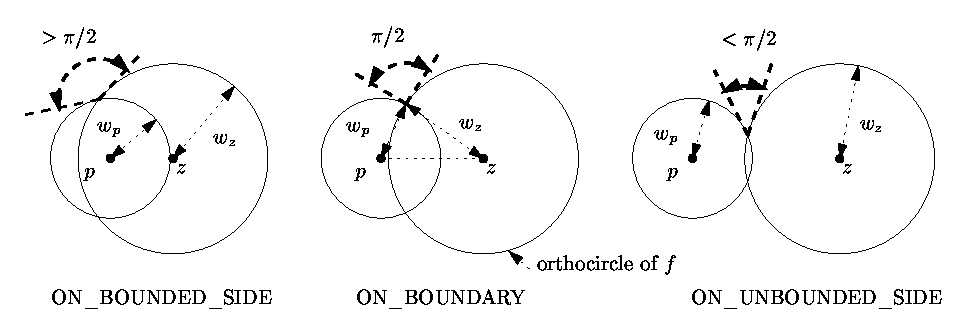
\includegraphics{sidedim2.eps} 
\end{center}
\end{ccTexOnly}
\caption{side\_of\_power\_circle.
\label{Triangulation3-fig-sidedim2}}
\begin{ccHtmlOnly}
<CENTER>
<img border=0 src="./sidedim2.gif" align=center
alt="side_of_power_circle"> 
</CENTER>
\end{ccHtmlOnly}
\end{figure} 

\ccMethod{Bounded_side
          side_of_power_sphere(Cell_handle c, const Weighted_point & p) const;}
{Returns the position of the weighted point $p$ with respect to the
power sphere of \ccc{c}. More precisely, it returns:\\
- \ccc{ON_BOUNDED_SIDE} if $\Pi({p}^{(w)}-{z(c)}^{(w)})<0$ where
${z(c)}^{(w)}$ is the power sphere of \ccc{c}. For an
infinite cell this means either that \ccc{p} lies strictly in the half
space limited by its finite facet and not containing any other point
of the triangulation, or that the angle 
between \ccc{p} and the power circle of the \textit{finite} facet of \ccc{c}
is greater than $\pi/2$. \\  
- \ccc{ON_BOUNDARY} if p is orthogonal to the power sphere of \ccc{c}
i.e. $\Pi({p}^{(w)}-{z(c)}^{(w)})=0$. For an infinite cell this means
that \ccc{p} is orthogonal to the power circle of its \textit{finite} facet.\\ 
- \ccc{ON_UNBOUNDED_SIDE} if $\Pi({p}^{(w)}-{z(c)}^{(w)})>0$
i.e. the angle between the weighted point \ccc{p} and the power sphere
of \ccc{c} is less than $\pi/2$ or if these two spheres do not
intersect. For an 
infinite cell this means that \ccc{p} does not satisfy either of the
two previous conditions. 
\ccPrecond{\ccVar.\ccc{dimension()} $=3$.}}

\ccMethod{Bounded_side
	  side_of_power_circle(const Facet & f, 
			const Weighted_point & p) const;}
{Returns the position of the point \ccc{p} with respect to the
power circle of \ccc{f}. More precisely, it returns:\\
--- in dimension~3:\\
-- For a finite facet,\\
\ccc{ON_BOUNDARY} if \ccc{p} is orthogonal to the power circle in the
plane of the facet,\\ 
\ccc{ON_UNBOUNDED_SIDE} when their angle is less than $\pi/2$,\\
\ccc{ON_BOUNDED_SIDE} when it is greater than $\pi/2$ (see
Figure~\ref{Triangulation3-fig-sidedim2}).\\ 
-- For an infinite facet, it considers the plane defined by the finite
facet of the cell \ccc{f.first}, and does the same as in
dimension~2 in this plane.\\
--- in dimension~2:\\
-- For a finite facet,\\
\ccc{ON_BOUNDARY} if \ccc{p} is orthogonal to the circle,\\
\ccc{ON_UNBOUNDED_SIDE} when the angle between \ccc{p} and the
power circle of \ccc{f} is less than $\pi/2$,
\ccc{ON_BOUNDED_SIDE} when it is greater than $\pi/2$.\\ 
-- For an infinite facet,\\
\ccc{ON_BOUNDED_SIDE} for a point in the open half plane defined by
\ccc{f} and not containing any other point of the triangulation,\\
\ccc{ON_UNBOUNDED_SIDE} in the other open half plane.\\
If the point \ccc{p} is collinear with the finite edge \ccc{e} of
\ccc{f}, it returns:\\
\ccc{ON_BOUNDED_SIDE} if $\Pi({p}^{(w)}-{z(e)}^{(w)})<0$, where
${z(e)}^{(w)}$ is the power segment of \ccc{e} in the line supporting
\ccc{e},\\ 
\ccc{ON_BOUNDARY} if $\Pi({p}^{(w)}-{z(e)}^{(w)})=0$,\\
\ccc{ON_UNBOUNDED_SIDE} if $\Pi({p}^{(w)}-{z(e)}^{(w)})>0$ .
\ccPrecond{\ccVar.\ccc{dimension()} $\geq 2$.}}

\ccMethod{Bounded_side
	  side_of_power_circle(Cell_handle c, int i, 
			const Weighted_point & p) const;}
{Same as the previous method for facet \ccc{i} of cell \ccc{c}.}

\ccMethod{Bounded_side
	  side_of_power_segment(Cell_handle c, const Weighted_point & p)
const;}
{In dimension~1, returns\\
\ccc{ON_BOUNDED_SIDE} if $\Pi({p}^{(w)}-{z(c)}^{(w)})<0$, where
${z(c)}^{(w)}$ is the power segment of the edge represented by
\ccc{c},\\
\ccc{ON_BOUNDARY} if $\Pi({p}^{(w)}-{z(c)}^{(w)})=0$,\\
\ccc{ON_UNBOUNDED_SIDE} if $\Pi({p}^{(w)}-{z(c)}^{(w)})>0$ .
\ccPrecond{\ccVar.\ccc{dimension()} $= 1$.}}

\begin{ccAdvanced}
\ccHeading{Checking}
\ccMethod{bool
          is_valid(bool verbose = false) const;}
{Checks the combinatorial validity of the triangulation and the
validity of its geometric embedding (see
Section~\ref{Triangulation3-sec-Valid}). Also checks that all the
power spheres (resp. power circles in dimension~2, power segments in
dimension~1) of cells (resp. facets in dimension~2, edges in
dimension~1) are regular. When \ccc{verbose}
is set to true, messages describing the first invalidity encountered
are printed.\\ This method is mainly a debugging help for the users of
advanced features.
}

\end{ccAdvanced}

%\ccSeeAlso

%% \ccExample

%% \ccIncludeExampleCode{examples/Triangulation3/Regular_triangulation_3_prog.C}

\end{ccRefClass}

% +------------------------------------------------------------------------+
%%RefPage: end of main body, begin of footer
% EOF
% +------------------------------------------------------------------------+

